\subsection{Swift}
Swift ist eine neue, von Apple entwickelte, Programmiersprache für die Entwicklung von iOS und Mac Apps. Sie ist eine Weiterentwicklung aus der Sprache Objective-C und kann deren Code problemlos ausführen. Laut Apple ist Swift rund 2,6 mal so schnell wie Objective-C.

\subsection{Übertragung}

\paragraph{Sockets}
Der erste Ansatz in diesem Projekt, war die Übertragung der Daten über Sockets. Diese können genutzt werden um sämtliche Daten bidirektional über Netzwerke zu senden. Ein Socket wird serverseitig an eine Adresse und einen Port gebunden. Ein Client kann sich zu einem diesen Socket verbinden und Daten austauschen. \\
Die Implementierung einer Socket-Verbindung funktioniert in Swift problemlos, allerdings ist sie mit einem großen Aufwand verbunden. Große Probleme stellt die Verschlüsselung der zu sendenden Daten dar. Diese müsste selbst implementiert werden. (QUELLEN !!!!). 
\begin{lstlisting}[caption =Implementierung einer Socketverbindung in Swift (Schematische Darstellung), language=C, frame=single, breaklines=true,columns=fullflexible, commentstyle=\color{gray}\upshape, captionpos=b, numbers = left]

private var inputstream : NSInputStream!
    private var outputstream : NSOutputStream!
    private var host : String = ""
    private var port : UInt32 = 0

func connect() {        
	// Initialisierung des Input- und Outputstreams
}

internal func stream(aStream: NSStream, handleEvent eventCode: NSStreamEvent) {
	// Behandeln der einzelnen Stream-Events

        switch (eventCode){
        case NSStreamEvent.ErrorOccurred:
		// Fehler beim Empfang oder Senden
        case NSStreamEvent.EndEncountered:
		// Ende der Übertragung
        case NSStreamEvent.HasBytesAvailable:
		// Es sind Daten auf dem Stream verfügbar
        case NSStreamEvent.OpenCompleted:
		// Stream erfolgreich geöffnet
        case NSStreamEvent.HasSpaceAvailable:
		// Space am Ende der Übertragung
        default:
        }
    }

\end{lstlisting}
Die vollständige Implementierung von mir ist auf Github einsehbar (https://github.com/hoedding/Studienarbeit-Anwendung/blob/master/iOS-App/Studienarbeit/ConnectServerTCP.swift).

\paragraph{HTTP}
Aufgrund der aufwändigen Implementierung und Schwierigkeiten mit der Verschlüsselung bei der Socketverbindung wurde als zweiter Ansatz die Übertragung der Daten im HTTP-Protokoll gewählt. Dieses Protokoll wird im Internet für die Daten- übertragung zu Webservern verwendet. Ein Webserver wartet auf eingehende Anfragen von Clients. Beim Verbindungsaufbau wertet er die Daten aus und antwortet dementsprechend. Eine Anfrage kann beliebige Daten enthalten. \\
In Swift ist die Funktionalität des Clients in der Klasse NSURLSession implementiert und ist einfach einzusetzen. Die Verschlüsselung findet automatisch statt, wenn eine Zieladresse mit dem Protokollidentifier 'https' beginnt.\\\\
Da ein HTTP-Request ein Asynchrone Request ist, muss der Methode sendMessageViaHttpPostWithCompletion() eine andere Methode (completionClosure : (s : NSString) -\textgreater ()) übergeben werden, die aufgerufen wird, wenn die Abfrage beendet ist. Mit dem Framwork 'IJReachability' kann überprüft werden ob eine Internetverbindung verfügbar ist und von welchem Typ (WLAN, Mobile) diese ist. 

\begin{lstlisting}[caption =Implementierung HTTP-Request in Swift, language=C++, frame=single, breaklines=true,columns=fullflexible, commentstyle=\color{gray}\upshape, captionpos=b, numbers = left]
func sendMessageViaHttpPostWithCompletion(message : NSString, completionClosure : (s : NSString) -> ()) {
    self.initServerConnection()
    var result : NSString = ""
    if !IJReachability.isConnectedToNetwork() {
	    return
    }
    let request = NSMutableURLRequest(URL: NSURL(string: server)!)
    request.HTTPMethod = "POST"
    let postString = "data=" + (message as String)
    request.HTTPBody = postString.dataUsingEncoding(NSUTF8StringEncoding)
    
    var configuration = NSURLSessionConfiguration.defaultSessionConfiguration()
    var session = NSURLSession(configuration: configuration, delegate: self, delegateQueue: NSOperationQueue.mainQueue())
    var task = session.dataTaskWithRequest(request) {
    data, response, error in
    
    if error != nil {
	    println("error=\(error)")
	    return
	}
    result = NSString(data: data, encoding: NSUTF8StringEncoding)!
    completionClosure(s: result)
    }
    task.resume()
}
\end{lstlisting}

Die vollständige Implementierung ist auf Github einsehbar (https://github.com/hoedding/Studienarbeit-Anwendung/blob/master/iOS-App/Studienarbeit/ConnectServerHTTP.swift)

\subsection{CoreData}
Mit CoreData wird eine Framework zur persistenten Speicherung von Daten geboten.Die Datenbank basiert auf einem tabellenbasierten relationalen Datenbankmodell. Grundsätzlich sollen hier die selben Daten wie in der Serveranwendung gespeichert werden. Die Entität 'Config' enthält folgende Attribute:

\begin{figure}[h]
	\begin{minipage}{0.5\textwidth}
		\centering
		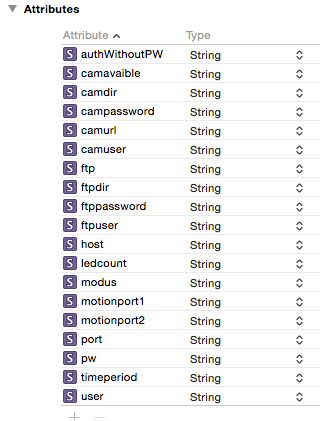
\includegraphics[width=\textwidth]{./data/entityconfig.png}
		\caption{Entität Config}
	\end{minipage}
\end{figure}

Um einen schnellen Zugriff auf die Daten zu ermöglichen wurden Methoden zum Lesen und Schreiben implementiert. Unter anderem mit der Methode changeValueWithEntityName() kann ein Eintrag geändert werden: 
\begin{lstlisting}[caption =Implementierung HTTP-Request in Swift, language=C++, frame=single, breaklines=true,columns=fullflexible, commentstyle=\color{gray}\upshape, captionpos=b, numbers = left]
func changeValueWithEntityName(entityName : String, key : String, value : AnyObject) {
    var err : NSError? = nil
    var appDel : AppDelegate = (UIApplication.sharedApplication().delegate as! AppDelegate)
    var context : NSManagedObjectContext = appDel.managedObjectContext!
    var request = NSFetchRequest(entityName: entityName)
    request.returnsObjectsAsFaults = false
    var result : Array = context.executeFetchRequest(request, error: &err)! as Array
    if (result.count == 1){
	    for res in result {
		    res.setValue(value, forKey: key)
	    }
    }
    context.save(&err)
    if (err != nil) {
	    println(err)
    }
}
\end{lstlisting}

\subsection{Konzept}
Beim Start der App soll die Verbindung zum Server aufgebaut werden. Hierbei sollen die Zugangsdaten überprüft werden und alle Daten synchronisiert werden. Das bedeutet es werden bei jeder Verbindung mit korrektem Login alle Konfigurationsdaten des Servers an den Client gesendet. Des weiteren wird der aktuelle Status der LEDs übertragen. \\
Nach dem Verbindungsaufbau ist es dem Benutzer möglich, den Modus des Systems zu verändern. Außerdem kann er alle anderen Funktionen in der App nutzen.

\begin{figure}[h]
	\begin{minipage}{\textwidth}
		\centering
		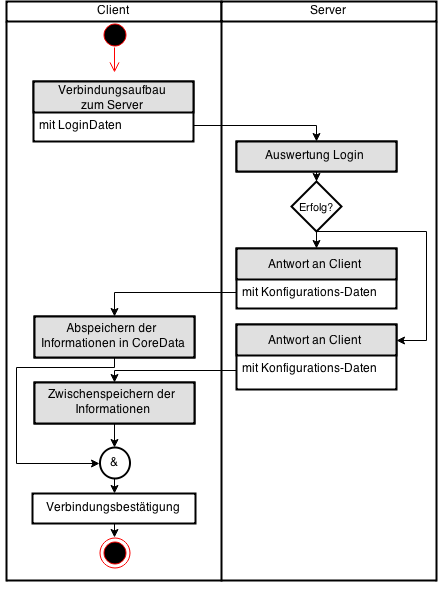
\includegraphics[width=0.6\textwidth]{./data/konzept.png}
		\caption{Konzept der Server-Client-Kommunikation}
	\end{minipage}
\end{figure}

\subsection{Aufbau}
In einer Standard iOS-App werden die einzelnen Seiten Klassenweise implementiert. In einem visuellen Editor können Grundelemente wie Buttons und Textfelder hinzugefügt werden. Diese werden über Outlets mit den zugehörigen Klasen verbunden und können direkt im Code angesprochen werden. Es wurden weitere Klassen für die Kommunikation mit der Serveranwendung und CoreData angelegt. Um zwischen den einzelnen Views zu wechseln, wird ein Menü verwendet, welches sich durch eine Wisch-Bewegung vom linken Rand öffnet. 

\paragraph{Framworks} Es wurden einige Frameworks eingesetzt:
\begin{itemize}
	\item \textbf{CryptoSwift:} Bietet viele Hashalgorithmen. 
	\item \textbf{VIPhotoView:} Notwendig für die Bildansicht im Archiv.
	\item \textbf{WhiteRacoon:} FTP-Verbindung und Management.
	\item \textbf{IJReachability:} Überprüft welche Internetverbindung vorhanden ist.
	\item \textbf{SideMenu:} Slide-Menü der Anwendung.
\end{itemize}

